\documentclass[12pt]{article}

\usepackage[letterpaper, margin=1in]{geometry}
\usepackage{tikz}
\usetikzlibrary{calc}
\usepackage{enumitem}
\usepackage{graphicx}
\usepackage{hyperref} % Add this package for hyperlinks
\pdfminorversion=7 % Allow inclusion of PDF version 1.7 files

\setlength{\parskip}{1em}
\setlength{\parindent}{0pt}

\begin{document}

\begin{titlepage}
    \centering
    \vfill
    \vspace*{2.5in}
    \begin{tikzpicture}[remember picture, overlay]
        \draw [line width=1pt, rounded corners=10pt] 
            ($(current page.north west) + (0.5in,-0.5in)$) rectangle 
            ($(current page.south east) + (-0.5in,0.5in)$);
    \end{tikzpicture}
    {\Huge\bfseries Capstone 2025 - Initial Proposal \par}
    \vspace{0.2in}
    {\LARGE Tolly Zhang \par}    
    \vspace{0.2in}
    {\LARGE December 20, 2024 \par}
    \vfill
\end{titlepage}

\newpage
\thispagestyle{empty}
\begin{center}
    \vspace*{\fill}
    \Large\textit{Nothing in this document is permanent and everything is potentially subject to change.}
    \vspace*{\fill}
\end{center}

\newpage
\pagenumbering{arabic}
\setcounter{page}{1}

\section{Project Overview}
\subsection{Background}

\subsubsection{Personal Significance}
I have a strong interest in aviation and autonomous systems, as well as many skills in engineering, electronics, and computer science. In November 2020 and May 2021, I had the opportunity to work on a project consisting of building a quadcopter drone. At the time, my resources and capabilities were limited. However, as time has passed, so has my knowledge as well as my access to resources. I hope to use this project as a way to further develop my skills and knowledge in these areas, and to create a system that can be used for real-world applications. A "passion project" like this would greatly benefit my portfolio and future career prospects.

\subsubsection{Current State of Aerial Delivery Systems}
Aerial delivery systems have evolved significantly, with companies like Zipline leading the U.S. drone-delivery industry. By 2024, drones completed around 14,000 deliveries daily worldwide, a number projected to reach 800 million annually by 2034.

Major players such as Amazon, Google, Walmart, DroneUp, and Matternet are actively developing and deploying drone delivery services. For instance, Amazon conducted its first drone delivery test in Italy in December 2024, using the MK30 drone capable of carrying up to five pounds and operating in light rain.

Aerial delivery systems offer the following advantages over traditional delivery methods:
\begin{itemize}
    \item Faster delivery times compared to traditional methods.
    \item Reduced operational costs due to lower energy consumption and labor expenses.
    \item Ability to access remote and rural areas without the need for extensive infrastructure.
    \item Environmentally friendly with lower carbon emissions per package delivered.
    \item Enhanced supply chain resilience, especially during emergencies or disruptions.
    \item Improved inventory management through frequent, small-scale deliveries.
\end{itemize}

However, current systems face several challenges, including:
\begin{itemize}
    \item Regulatory hurdles
    \item Safety concerns
    \item Public apprehension
    \item Limited payload capacity
    \item Vulnerability to adverse weather
    \item High operational costs
\end{itemize}

This project aims to address these challenges by developing an advanced aerial package delivery system that overcomes the limitations of existing solutions.

\subsection{Objective}
The objective of this project is to \textbf{design and develop an advanced aerial package delivery system} that can \textbf{efficiently transport small to medium-sized payloads over varying distances}. The system will be composed of four key components:
\begin{enumerate}
    \item \textbf{Dynamic Aerial Mobility System (DAMS)} \\
    Ensures versatile and efficient flight capabilities.
    \item \textbf{Payload Retrieval and Deployment Module (PRDM)} \\
    Manages secure and autonomous payload handling.
    \item \textbf{Automated Flight Navigation System (AFNS)} \\
    Provides precise and autonomous navigation.
    \item \textbf{Adaptive Flight Control Interface (AFCI)} \\
    Facilitates user-friendly control and monitoring.
\end{enumerate}

\subsection{Key Performance Indicators (KPIs)}
The success of the project will be measured using the following key performance indicators.

\textit{The specific method of measurement for each KPI is yet to be determined.}
\begin{itemize}
    \item Drop-off accuracy (i.e., distance from the intended delivery location).
    \item Mission success rate (i.e., the ratio between the number of successful missions and the total number of attempted missions).
    \item Average distance traveled per unit of battery capacity (km/wh).
    \item Maximum operational time per full charge under normal conditions.
    \item Time and energy required to switch between VTOL and fixed-wing modes.
    \item Maximum payload weight the system can transport reliably.
    \item Maximum allowed deviation from center of gravity during flight with varying payload distributions.
    \item Time required to autonomously and reliably pick up or drop off a payload.
    \item Percentage of successful obstacle detections and avoidances during flight.
    \item Time reduced in delays for simultaneous delivery missions.
    \item Average time latency for the Adaptive Flight Control Interface (AFCI) to execute commands.
    \item Time required for an operator to prepare and verify a device for flight.
    \item User satisfaction scores on a scale of 1-10 based on ease of use and reliability.
    \item Percentage of successful landings after a simulated single/multi-motor or system failure.
    \item Performance under various weather conditions.
    \item Percentage of correctly identified and reported system errors.
    \item Average total cost of operation per single delivery.
    \item Average time between required repairs or system maintenance tasks.
\end{itemize}

\subsection{Stakeholders and Roles}
The following stakeholders will be involved in the project:
\begin{enumerate}
    \item \textbf{Tolly Zhang} (Project Manager) \\
    Responsible for overall project coordination, planning, and execution. Roles include:
    \begin{itemize}
        \item Developing, building, and testing all components of the system.
        \item Ensuring compliance with project requirements and deadlines.
        \item Managing the project budget and resources.
        \item Overseeing the integration of the system components.
    \end{itemize}
    \item \textbf{Mr. Michael Ho (and other SA teachers)} (Academic Advisor(s)) \\
    Provides guidance and support throughout the project. Roles include:
    \begin{itemize}
        \item Monitoring the project's progress and providing feedback.
        \item Providing resources as necessary for the project's success.
    \end{itemize}
\end{enumerate}
There are a few other potential resources that may be involved in the project, shown below.

\textit{All aid from external resources will be acknowledged and credited appropriately.}
\begin{itemize}
    \item \textbf{Academic Colleagues} \\
    May be consulted based on expertise to assist in the development of specific components. Specific people are yet to be decided upon.
    \item \textbf{Subject Matter Expert (SME)} \\
    May be consulted for assistance with high-level technical challenges. The SME(s) will be identified and contacted as needed.
    \item \textbf{Manufacturing Partners} \\
    May be engaged to produce specific components or subsystems. Partners will be selected based on their expertise and capabilities.
    \item \textbf{Generative AI Models} \\
    May be used to assist in the building of certain system components. The specific models and their developers will be identified as needed.
\end{itemize}

\subsection{Timeline}
Forenote: The project is \textit{not} expected to be completed by the Capstone presentation in September 2025. The timeline below outlines the key milestones for the project:
\begin{itemize}
    \item \textbf{January–February 2025}:
    \begin{itemize}
        \item Research, ideation, and initial concept development.
        \item Prototyping of different systems in the DAMS and PRDM.
    \end{itemize}
    \item \textbf{March–June 2025}:
    \begin{itemize}
        \item Component selection for the DAMS and PRDM.
        \item CAD development and simulation of the system architecture.
    \end{itemize}
    \item \textbf{July 2025}:
    \begin{itemize}
        \item Manufacturing and assembly of the designed components for the DAMS and PRDM.
        \item Initial testing of individual components and subsystems.
    \end{itemize}
    \item \textbf{August–September 2025}:
    \begin{itemize}
        \item Integration of the components, testing, and initial flight trials for the DAMS and PRDM.
    \end{itemize}
    \item \textbf{October–November 2025}:
    \begin{itemize}
        \item Refinement of DAMS and PRDM.
        \item Development of the AFNS and AFCI.
    \end{itemize}
    \item \textbf{December 2025}:
    \begin{itemize}
        \item Integration of all components and systems.
        \item Final testing and evaluation of the complete system.
    \end{itemize}
\end{itemize}

\newpage
\section{Concept Development}
\subsection{System Architecture}

\subsubsection{Dynamic Aerial Mobility System (DAMS)}
The DAMS will feature a Vertical Take-Off and Landing (VTOL) flight system, capable of switching between VTOL and fixed-wing flight modes. The VTOL mode will be used for takeoff and landing, while the fixed-wing mode will facilitate efficient cruising. The DAMS integrates the \textbf{Dynamic Flight Control Unit}, which ensures smooth transitions between flight modes using \textbf{actuators} to control components such as rudders, elevators, and ailerons. Sensors, including IMUs (Inertial Measurement Units) and LIDAR, will provide real-time feedback for stability and maneuverability during flight. The DAMS will also interface with the \textbf{Automated Flight Navigation System (AFNS)} for autonomous flight control.

\subsubsection{Payload Retrieval and Deployment Module (PRDM)}
The PRDM will be responsible for the autonomous retrieval and deployment of payloads. It will utilize the \textbf{Payload Control Unit} to manage and control various components for payload operations. Key features will include:
\begin{itemize}
    \item An opening/closing door for payload access, controlled by actuators.
    \item A clamp mechanism to securely hold the payload during flight.
    \item A winch mechanism for raising and lowering the payload during retrieval and deployment.
    \item Proximity and weight sensors to monitor payload positioning and distribution, providing real-time data to the DAMS to ensure stability and balance.
\end{itemize}
The PRDM will work in coordination with the \textbf{DAMS} to ensure the aircraft maintains stability and efficient operation during payload operations.

\subsubsection{Automated Flight Navigation System (AFNS)}
The AFNS will determine the optimal flight path from the source to the destination, leveraging data from onboard sensors such as GPS, cameras, and LIDAR. It will provide precise navigational instructions to the DAMS and coordinate with other onboard systems for efficient path planning. The AFNS will also support multi-aircraft management, enabling the simultaneous coordination of multiple deliveries and flight routes.

\subsubsection{Adaptive Flight Control Interface (AFCI)}
The AFCI will serve as the human-machine interface, allowing the operator to interact with both the AFNS and the DAMS. It will feature:
\begin{itemize}
    \item Multiple modes of operation, including manual, semi-autonomous, and autonomous.
    \item Input devices such as screens, keyboards, mice, and controllers.
    \item A speech control interface for hands-free operation, integrated with an audio recorder and speaker system.
    \item A heads-up display (HUD) for providing real-time telemetry and flight data to the operator.
\end{itemize}
The AFCI will ensure that operators have full control and oversight during all phases of operation, while enabling user-friendly interaction with the system.

\noindent\rule{\textwidth}{0.4pt}

Below is a diagram displaying the correlations between the four different components (created using \href{https://www.diagrams.net/}{diagrams.net}):

\begin{figure}[h]
    \centering
    \begin{tikzpicture}
        \node[inner sep=0pt] (diagram) at (0,0) {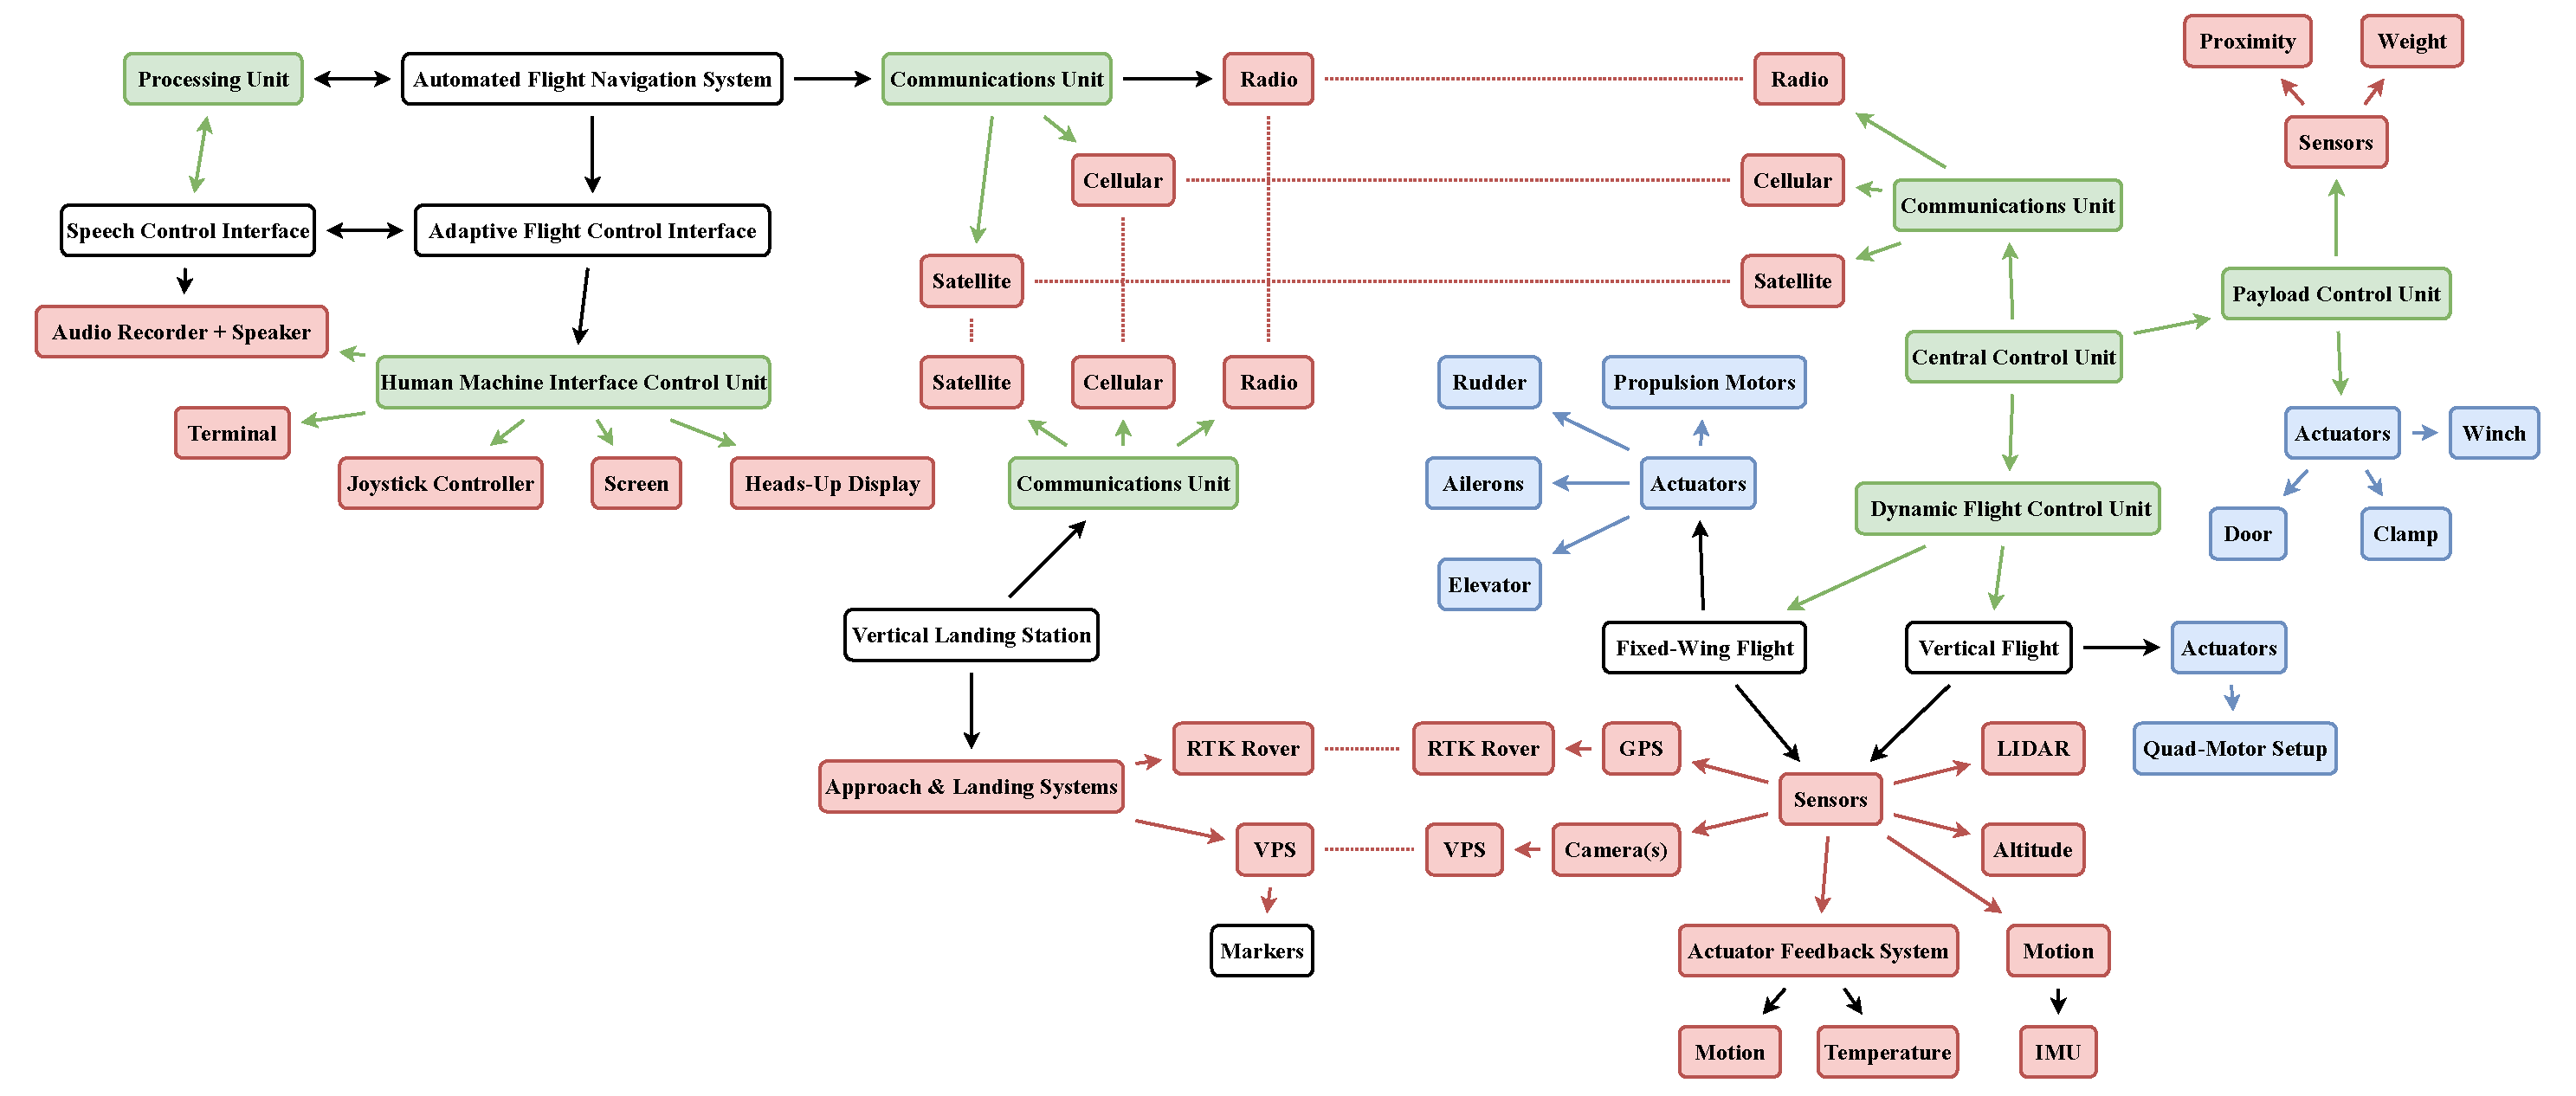
\includegraphics[width=\textwidth]{resources/system-architecture.drawio.pdf}};
        \draw [line width=1pt, rounded corners=10pt] 
            (diagram.north west) rectangle 
            (diagram.south east);
    \end{tikzpicture}
    \caption{System Architecture Diagram}
\end{figure}

\newpage

\section{Development Approach}

Below is a brief overview of the development approach for each component of the system:

\subsection{Dynamic Aerial Mobility System (DAMS)}
\subsubsection{Fixed Wing Mode}
The fixed-wing mode will be optimized for efficient cruising and long-range flight.
The following aspects will be considered during the development of the fixed-wing mode:
\begin{itemize}
    \item \textbf{Aspect Ratio} (Ratio of wing span to mean chord length)
    \item \textbf{Airfoil} (Shape of the wing cross-section)
    \item \textbf{Sweep Angle} (Angle of the wing relative to the aircraft's longitudinal axis)
    \item \textbf{Dihedral Angle} (Upward angle of the wings from horizontal)
    \item \textbf{Required Thrust} (Amount of thrust needed for flight)
    \item \textbf{Aerodynamics} (Study of the motion of air and its interaction with the aircraft)
    \item \textbf{Control Surfaces} (Movable surfaces used to control the aircraft's attitude)
    \item \textbf{Stall Speed} (Minimum speed at which the aircraft can maintain level flight)
    \item \textbf{L/D Ratio} (Lift-to-drag ratio, a measure of aerodynamic efficiency)
    \item \textbf{Wing Loading} (Weight of the aircraft divided by the wing area)
    \item \textbf{Tail Configuration} (Design and arrangement of the tail surfaces)
    \item \textbf{Material Selection} (Choice of materials for constructing the aircraft)
\end{itemize}

Multiple iterations of the fixed-wing design will be tested using simulation software to optimize performance and efficiency before physical prototyping.

\subsubsection{VTOL Mode}
The VTOL mode will be optimized for vertical takeoff and landing, providing stability and control during these critical phases of flight.
The following aspects will be considered during the development of the VTOL mode:
\begin{itemize}
    \item \textbf{Thrust Vectoring} (Control of thrust direction for maneuverability)
    \item \textbf{Propeller Configuration} (Number and arrangement of propellers for lift)
    \item \textbf{Material Selection} (Choice of materials for constructing the aircraft)
\end{itemize}

The VTOL mode will be integrated with the fixed-wing mode to ensure mechanical and aerodynamic compatibility, allowing for seamless transitions between flight modes.

\subsubsection{General Flight}
The DAMS will be designed to seamlessly transition between fixed-wing and VTOL modes, ensuring smooth and efficient flight operations.

The following aspects will be considered during the development of the general flight capabilities:
\begin{itemize}
    \item \textbf{Propulsion System} (Engines, motors, or rotors used for vertical lift)
    \item \textbf{Control Surfaces} (Ailerons, elevators, rudders, and flaps for maneuvering)
    \item \textbf{Transition Mechanism} (Mechanism for switching between VTOL and fixed-wing modes)
    \item \textbf{Stability Augmentation} (Systems to enhance stability during takeoff and landing)
    \item \textbf{Power Source} (Battery or fuel system for providing energy)
    \item \textbf{Safety Features} (Redundant systems, fail-safe mechanisms, and failure detection and mitigation)
    \item \textbf{Payload Handling} (Integration with the PRDM for payload operations)
\end{itemize}

The DAMS will undergo rigorous testing to ensure reliability, stability, and efficiency during flight operations.

\subsection{Payload Retrieval and Deployment Module (PRDM)}
The PRDM will be designed to autonomously handle payloads, ensuring secure and efficient retrieval and deployment.

The following aspects will be considered during the development of the PRDM:
\begin{itemize}
    \item \textbf{Payload Handling Mechanism} (Clamps, winches, and doors for payload operations)
    \item \textbf{Payload Sensors} (Proximity sensors, weight sensors, and cameras for monitoring payloads)
    \item \textbf{Payload Control Unit} (System for managing payload operations)
    \item \textbf{Payload Security} (Mechanisms to secure payloads during flight)
    \item \textbf{Payload Compatibility} (Design considerations for various payload sizes and shapes)
    \item \textbf{Payload Integration} (Integration with the DAMS for stability and balance)
\end{itemize}

The PRDM will be tested under various conditions to ensure reliable and efficient payload handling, with a focus on safety and stability during flight operations.

\subsection{Automated Flight Navigation System (AFNS)}
The AFNS will be designed to provide precise and autonomous navigation for the aircraft, ensuring efficient flight paths and mission success. It will be a primarily software-based, on-ground system that interfaces with the DAMS and PRDM for flight control and payload operations.

The following aspects will be considered during the development of the AFNS:
\begin{itemize}
    \item \textbf{Path Planning} (Optimal route selection based on mission requirements)
    \item \textbf{Obstacle Avoidance} (Detection and avoidance of obstacles during flight)
    \item \textbf{Mission Management} (Coordination of multiple aircraft and deliveries)
    \item \textbf{Real-Time Data Processing} (Processing of sensor data for navigation and control)
    \item \textbf{Communication Protocols} (Data exchange between the AFNS and DAMS)
    \item \textbf{Autonomous Decision-Making} (Automated responses to changing flight conditions)
    \item \textbf{Redundancy and Fail-Safe Mechanisms} (Backup systems and safety features)
\end{itemize}

The DAMS will be programmed to operate independently in case of a failure in the AFNS, and vice versa. The AFNS will be tested in simulation and real-world scenarios to ensure reliable and efficient navigation under various conditions.

\subsection{Adaptive Flight Control Interface (AFCI)}
The AFCI will be designed to provide a user-friendly interface for operators to interact with the system, ensuring ease of use and oversight during flight operations.

The following aspects will be considered during the development of the AFCI:
\begin{itemize}
    \item \textbf{User Interface Design} (Layout, controls, and feedback mechanisms for operators)
    \item \textbf{Input Devices} (Screens, keyboards, controllers, and speech recognition systems)
    \item \textbf{Telemetry and Data Display} (Real-time flight data and system status information)
    \item \textbf{Control Modes} (Manual, semi-autonomous, and autonomous control options)
    \item \textbf{Safety Features} (Emergency stop, return-to-home, and system diagnostics)
    \item \textbf{Integration with AFNS} (Communication and data exchange with the AFNS)
\end{itemize}

The AFCI will be tested for usability, reliability, and efficiency, with a focus on operator satisfaction and system performance during flight operations.

\subsection{Required Resources}
The development of the system will require the following resources:
\begin{enumerate}
    \item \textbf{Hardware Components} (Sensors, actuators, motors, controllers, batteries, and structural materials)
    \item \textbf{Software Tools} (CAD software, simulation tools, programming languages, and development environments)
    \item \textbf{Manufacturing Facilities} (3D printers, CNC machines, and other fabrication equipment)
    \item \textbf{Testing Environments} (Indoor and outdoor testing areas, flight simulators, and safety equipment)
    \item \textbf{Technical Expertise} (Engineering, electronics, and computer science knowledge)
    \item \textbf{Funding} (Budget for purchasing components, materials, and resources)
\end{enumerate}

\section{Conclusion}
The proposed project aims to develop an advanced aerial package delivery system that overcomes the limitations of existing solutions. By integrating the Dynamic Aerial Mobility System (DAMS), Payload Retrieval and Deployment Module (PRDM), Automated Flight Navigation System (AFNS), and Adaptive Flight Control Interface (AFCI), the system will provide efficient and reliable transport of small to medium-sized payloads over varying distances.
\end{document}
